\section{Testing}

The demodulation algorithm was tested by coding the algorithm in C (as a console
application) and instrumenting it to display variables,
save arrays to files, and benchmark the various stages.
KissFFT is used as the FFT.
A GPU would be much faster and will be used in further studies.

\subsection{Demodulation to Image}

The demodulation algorithm looks at the signal bandwidth between about
$\gamma F_S/5$ and $\gamma F_S/2$ where $\gamma$ is between 0.25 and 1.

Figure \ref{fig:chirpTest1} shows a spectrogram image of a noisy test signal
with R on the vertical axis.
$R=-0.2$ is at the top and $R=-0.78$ is at the bottom.
The output rates for each R are normalized (stretched at the low end)
to fit the image.
This gives the top of the image a fuzzy appearance.
A test signal was used to demonstrate detection of a chirp at
$R=-0.5$ and $N=4096$.
The chirp amplitude is 1/10 of the noise amplitude.
\begin{figure}
  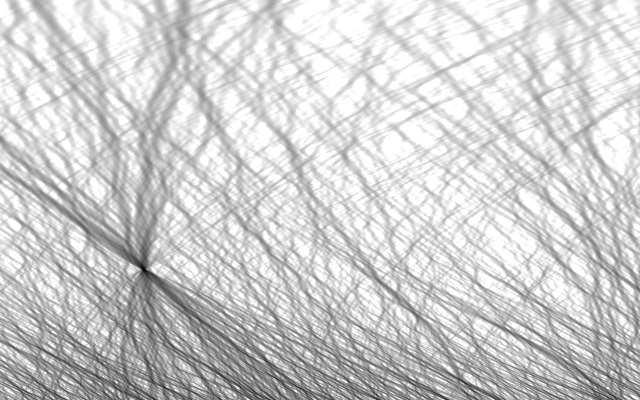
\includegraphics[width=\linewidth]{../source/chirp42m.jpg}
  \caption{Chirp power 20dB below noise.}
  \label{fig:chirpTest1}
\end{figure}

Noise has a cobweb-like look. A chirp shows up as a peak among the cobwebs.
To pick the chirp out of this mess, the peak is stored for each R value.
Figure \ref{fig:chirpRvalues1} shows the peak R values for a test chirp with a
power level 20, 25 and 30 dB below random noise.
\begin{figure}
  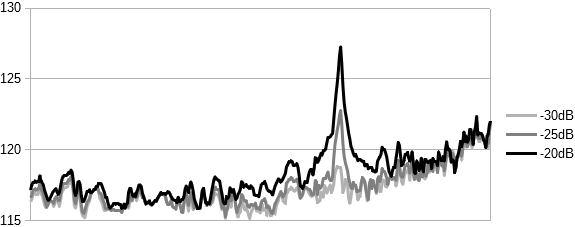
\includegraphics[width=\linewidth]{../source/Rpeaks.png}
  \caption{Peak power versus R}
  \label{fig:chirpRvalues1}
\end{figure}

